% !TeX spellcheck = da_DK
\subsection{Feedbackkonfiguration}
\subsubsection{Teori og design}
Jævnfør \ref{Komparatorafsnit} på side \pageref{Komparatorafsnit} anvendes en komparator til at sammenligne to inputspændinger. Komparatoren der anvendes er af typen LM311. Ved denne type placeres en 100n kondensator ved inputtet for at gøre komparatoren mere præcis og undgå svingninger\cite{Instruments2015}. Der vil blive anvendt flere komparatorer og i dette tilfælde tilkobles komparatorernes output en LED, en vibrator, en modstand og den positive spændingsforsyning ($+V_{cc}$). I komparatorernes ikke-inverterende terminaler tilsluttes outputtet fra forrige blok, hvor inputtet i de inverterende terminaler fungerer som referencespænding, der forsyner med de beregnede tærskelværdier. Komparatorerne kan derfor have to forskellige outputs afhængig af inputspændingen. Hvis inputsignalet ligger udenfor de beregnede tærskelværdier vil outputtet være $0V$ og LEDerne samt de to vibratorer vil ikke blive aktiveret. Er inputtet derimod indenfor de beregnede tærskelværdier, vil outputtet svare til ground, da strømmen fra $+V_{cc}$ vil løbe igennem komparatorerne og derefter til ground\fxnote{det vil vel løbe til komparatorens emitter terminal }. Derved opnås et spændingsfald over den positive (anode) og negative (katode) pol for LEDerne og vibratorerne på en værdi, der ligger over det minimale spændingsfald, der kræves for en aktivering. LEDerne og vibratorerne vil derved blive aktiveret og fungere som feedback til patienten. \\

Til den visuelle del af feedbackkonfigurationen anvendes LEDer. En LED har to terminaler; en anode og en katode. Når en ideel LED tændes skyldes det, at der løber strøm fra anoden til katoden og der vil her være et spændingsfald over LEDen på 0V. Dette kaldes fremadgående spændings. Når strømmen løber fra katoden til anoden vil LEDen være slukket, da der ideelt ikke løber strøm igennem kredsløbet.... \fxnote{mere burde tilføjes.} 


\noindent\textbf{Design af feedbackkonfiguration} \\
LEDernes katode tilkobles komparatorens output, imens anoden tilkobles $+V_{cc}$. Jævnfør kravspecifikationerne i afsnit \ref{KomparatorAfs} på side \pageref{KomparatorAfs} skal LEDerne aktiveres på fem forskellige stadier. Til denne aktiveren anvendes otte komparatorer, da det første stadie, indeholdende den grønne LED, både har en positiv og negativ tærskelværdi og derfor kræver to komparatorer. De valgte tærskelværdier kan designes på forskellige måder hhv. som to spændingstræer eller otte spændingsdelere, hvoraf der er fordele og ulemper ved begge metoder. I dette projekt anvendes otte spændingsdelere, hvormed to indgår i en vindues-komparatorkonfiguration for den grønne LED, og de seks resterende fungerer som almindelige komparatorer, der aktiveres over en bestemt tærskelværdi. Fordelen ved at vælge dette design er, at modstandene i et spændingstræ påvirker hinanden, hvilket kan ændre tærskelværdierne, hvis én af modstandene ikke fungerer optimalt. Ulempen ved at anvende spændingsdelere er, at der benyttes flere modstande ved denne konfiguration. Feedbackkonfigurationen kan inddeles i to dele; en for hældning i hhv. positiv og negativ retning. De otte spændingsdelere udgøres af i alt $12$ modstande (R$1$-R$12$). Derudover består kredsløbet af en spændingsreference ($+V_{ref}$) på $2.5$V og syv modstande (R$13$-R$19$) mellem LEDerne samt vibratorerne og $+V_{cc}$. Modstandene(R$13$-R$14$, R$16$-R$17$ og R$19$) sikre at batteriet ikke drænes og bestemmer mængden af strøm til LEDerne. Vindues-komparatorkonfigurationen designes ved at placere en LED (D$3$) i emitter-terminalen på komparatorerne (U$3$) og collector-terminalen komparatorerne (U$4$). Feedbackkonfigurationen fremgår af \figref{fig:komparator_uden_vaerdi} 

\begin{figure}[H] 
	\centering
	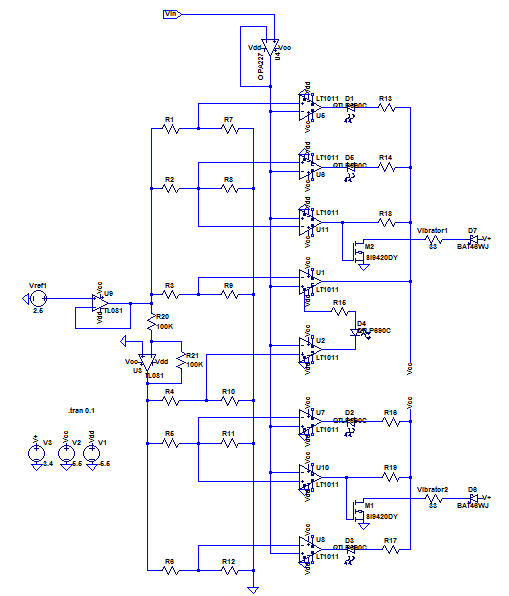
\includegraphics[scale=0.7]{figures/cProblemloesning/komparator_uden_vaerdi.PNG}
	\caption{På figuren ses feedbackkonfigurationen, hvor kredsløbet består af to dele; en for hældning i positiv og negativ retning. Der er konstrueret en vindues-komparatorkonfigurationen designet vha. komparatorerne (U$3$-U$4$) for den grønne LED, der anvender en tærskelværdi fra hhv. den negative og positive del af kredsløbet. Kredsløbet er konstrueret i LTspice.}
	\label{fig:komparator_uden_vaerdi}
\end{figure}

%%%%%%%%%%%%%%%%%%%%%%%%%%%%%%%%%%%%%%%%%%%%%%%%%%%%%%%%%%%%%%%

\noindent\textbf{Beregning af tærskelværdier og modstandene R$1$-R$12$} \\
Det ønskes, at LEDerne skal lyse ved bestemte kropshældninger, dvs. ved bestemte tærskelværdier. Inputsignalet afhænger af den pågældende hældningsgrad, hvilket for komparatoren vil være en bestemt spænding. Komparatorens tærskelværdierne kan beregnes, da værdien i volt pr. grad i hhv. positiv og negativ retning, jævnfør \eqref{taerskelvaerdi_pr_grad} i pilotforsøget i bilag \ref{Pilotforsoeg} på side \pageref{Sec_Pilot_Data}, samt forstærkningsværdien af signalet fra forrige blokke, opsamlings- og tilpasningsblokken, er kendte værdier. Jævnfør tærskelværdierne i afsnit \ref{Komparatorafsnit} på side \pageref{Komparatorafsnit} beregnet ud fra følgende formel:
\begin{equation}\label{pr_grad} 
\text{Tærskelværdi i positiv retning} = \frac{0.0037\text{V}*9.1*3.6*\text{hældningsgrad}} = tærskelværdi
\text{Tærskelværdi i negativ retning} = \frac{0.0036\text{V}*9.1*3.6*\text{hældningsgrad}} = tærskelværdi
\end{equation}

De udregnede tærskelværdier fremgår af \figref{taerskelvaerdier}. 
\begin{figure}[H]
	\centering
	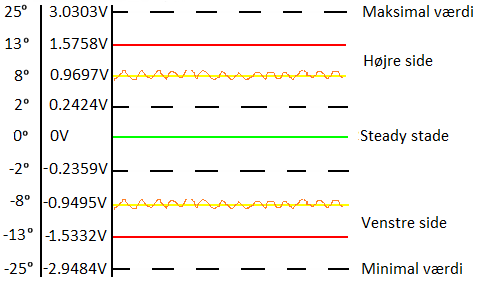
\includegraphics[scale=1.]{figures/cProblemloesning/Taerskelvaerdier.PNG}
	\caption{På figuren fremgår de beregnede tærskelværdier og hvilket farve, der lyser ved de de enkelte tærskler.}
	\label{fig:taerskelvaerdier}
\end{figure}


Der anvendes en spændingsreference, bestående af en regulator, der kan levere en konstant spænding på $2.5$V til feedbackkonfigurationen jævnført \ref{subsec:Spaendingsref_Komparator} på side \pageref{subsec:Spaendingsref_Komparator}. Eftersom spændingen ved anvendelse af et batteri vil falde som funktion af tiden benyttes spændingsreferencen, så denne kan holde en fast referencespænding i kredsløbet. Eftersom spændingsreferencen også skal anvendes til de negative tærskelværdier benyttes en inverterende forstærker med et gain på $1$ i designet af feedbackkonfigurationen, hvilket fremgår af figur \figref{fig:komparator_uden_vaerdi}. Ved denne konfiguration vendes signalet, uden at blive forstærket, og kan på denne måde benyttes som referencespænding til negative inputspændinger.


For at bestemme R$1$-R$12$ i spændingsdelerne, så LED-dioderne lyser ved de ønskede tærskelværdier defineres R$1$ til en bestemt værdi. I dette tilfælde fastsættes R$1$ til at være $10$K$\Omega$. Denne værdi er også gældende for R$2$-R$6$, da der benyttes en spændingsdeler for hver tærskelværdi. Derudover er de ønskede tærskelværdier ($V_out$) og spændingsreferencen ($V_in$) også kendte værdier og R$7$-R$12$ kan dermed udregnes vha. den generelle formel for en spændingsdeler jævnført \eqref{eq:Spaendingsdeler} i afsnit \ref{subsec:Spaendingsref} på side \pageref{subsec:Spaendingsref}. 

Dette medfører at R$7$-R$12$ giver følgende resultater:\\
R$7$ = $16821\Omega$ \\
R$8$ = $6285\Omega$ \\
R$9$ = $1068\Omega$ \\
R$10$ = $783\Omega$ \\
R$11$ = $6039\Omega$ \\
R$12$ = $15765\Omega$ \\

\fxnote{Der er implementeret en buffer samt en inverterende forstærker for at sikre en lav outputimpedans samt give en negativ referencespændingen, så hældning i den negative retning kan detekteres og gør kredsløbet mere stabilt. - hvordan skal jeg lige skrive dette ind i teksten?}


%%%%%%%%%%%%%%%%%%%%%%%%%%%%%%%%%%%%%%%%%%%%%%%%%%%%%%%%

\noindent\textbf{Beregning af R$13$-R$17$ modstande for aktivering af LED} \\
Jænvfør kravspecifikationerne i afsnit \ref{KomparatorAfs} på side \pageref{KomparatorAfs} for komparatoren skal forsyningsspændingen være $5.5$V. De anvendte LEDer i systemet er: en grøn L-$53$LG $5$mm (D$3$), to røde L-$53$LI $5$mm (D$1$ og D$5$) og to gule L-$53$LY $5$mm (D$2$ og D$4$) \fxnote{rettes til efter billedet}. Lederne kræver en minimum spænding på $2$mA for at lyse, men det vurderes, at der skal benyttes ca. $20$mA for tydeligt lys \fxnote{på baggrund af hvilken vurdering - ud fra hvad?}.  Spændingsfaldet over LED-dioderne ligger maksimalt i intervallet $2.0$V til $2.2$ V (rød: $2.0$, gul: $2.1$ og grøn: $2.2$), men typisk mellem $1.7$V-$1.9$V. LED-dioderne skal derudover forsynes med $2$mA for at fungere, men kan forsynes op til \fxnote{Tjek og 150mA er rigtigt}$150$mA, før de brændes af. LEDerne forsynes af en $5.5$V spændingsforsyning og tilkobles, som sagt, tilhørende modstande for bla. at undgå at LED-dioderne brænder af. Spændingsfaldet over dioderne samt den spænding LEDerne som minimum skal bruge for at lyse er kendte værdier, dvs. modstandene R$12$-R$17$ kan derfor findes vha. Ohms lov. Nedenstående udregning beregnet en værdi af modstandene, hvis spændingsforsyningen forsynerkredsløbet med $5.5$V og LEDernes minimale spænding for at aktiveres:

\begin{equation}
R = \dfrac{5.5V - 2.2V}{0.02A} = 165\Omega
\end{equation}
\noindent Dermed sættes modstandene R$12$-R$17$ alle til $165\Omega$ for at sikre, at der er tilstrækkeligt med strøm i kredsløbet til at dioderne kan lyse, uden at de brændes af eller at batterierne drænes. Opsætningen af LED-dioderne fremgår af figur \figref{fig:komparator_visuel}. \fxnote{Jeg ved ikke om modstandene R$13$-R$17$ passer til billedet, da det ikke passer ift. tabel 3.22}

%%%%%%%%%%%%%%%%%%%%%%%%%%%%%%%%%%%%%%%%%%%%%%%%%%%%%%%%%%%
\noindent\textbf{Somasensorisk feedback kredsløb} \\
Til det somasensoriske feedback kredsløb bruges der vibratorer, til at give feedbacken. En vibrator er en elektrisk motor, som kan bringe en masse i svingninger og derved skabe vibrationer
 \cite{Radaktionen2009}. Der er brugt en vibrator fra Jinlong Machinery \& Electronics Co. med produkt nummer, $28821$. Vibratoren har et drift arbejdsområde i $2.7-3.3$V, som typisk ligger på $3$V, men starter ved $2.3$V. Derfor skal virbratoren have en spændingsforsyning på $3$V.  Desuden er startstørmmen $120$mA, og når motoren kører er driftstrøm på $90$mA. Vibrationen sker herefter med en frekvens på $10-55$Hz afhængig af forsyningsspænding samt strøm. For at patienten kan have vibratorene placeret på hænderne, så er der brugt en vibrator med dimensionerne; $1$cm i diameter og $0.27$cm i tykkelse.  \fxnote{Sæt datablad som kilde} 
 
 Vibratoren vil indgår som en del af feedback blokken jævnført \ref{KomparatorAfs} på side \pageref{KomparatorAfs}. For at opnå et tilstrækkeligt størmniveau skal der bruges en transistor (BS$170$), for at generer mere strøm. Transistoren er placeret mellem vibratoren og komparatoren. Denne konfigration er udarbejde således at transistoren vil blive tændt og vibratoren aktiveres når komparatoren er slukket, modsat de komaparator konfigurationer som bruges ved LED. Dette skyldes at når komparatoren er tændt vil den trække strømmen  \fxnote{Ved ikke helt om det er strøm eller spænding} som er tilkoblet i et knudepunkt mellem komparatorens collector terminal og trasistorens gain terminal. Denne strøm kommer fra en spændingsforsyning på $5.5$V, hvor der desuden er placeret en $100$K modstande, der sørger for at konfigurationen bruger mindre størm, end ved brug af en mindre modstand. Når komparatoren slukker vil spændingen aktivere transistoren og der vil derfor dannes forbindelse mellem transistorens drain og source terminal og vibratoren aktivres. Spændingsforsyningen til vibratoren er $3.4$V for kommer fra spændingsregulatoren. Vibratoren skal forsynes med $3$V og derfor er der indsat en schottky diode (BAT$41$), hvor der sker et spændingsfald afhængig af strømmen som løber igennem dioden og da spændingsfaldet ikke er så stort vil der forekomme meget strøm. Derved bliver spændingen nedsat til under $3$V. Denne spændingsforsyning på $3.4$V vil blive aktiveret når komparatoren er slukket og der er forbindelse mellem transistorens drain og source terminal, da strømmen kan løbe til ground i source terminalen. 

\fxnote{Indsæt figur at vibrator kredsløbet i komparator konfigurationen}

\subsubsection{Simulering}
\noindent\textbf{Simulering af visuel komparatorkonfiguration} \\
Til simulering af den visuelle komparatorkonfiguration anvendes komparatorer af typen LT$1011$, da operationsforstærkerne til det reelle kredsløb er af denne type. For at udføre en simulering af den visuelle komparatorkonfiguration tilkobles kredsløbet et sinus-signal, der svinger mellem $\pm3$V. Dette gøres for at simulere signalet, der kommer fra den forrige blok, hvor arbejdsområdet er på $\pm3$V. Under simuleringen i LTspice testes det, hvorvidt den visuelle komparatorkonfiguration opfylder de opstillede specifikke krav, jævnfør kravspecifikationerne i afsnit \ref{KomparatorAfs} på side \pageref{KomparatorAfs}. Simuleringen af den visuelle komparatorkonfiguration fremgår af figur \figref{fig:komparator_visuel_simulering_samlet}. \fxnote{Vi kan starte med at simulere tærskelværdier og derefter hvordan komparatoren fungerer.}
\begin{figure}[H]
	\centering
	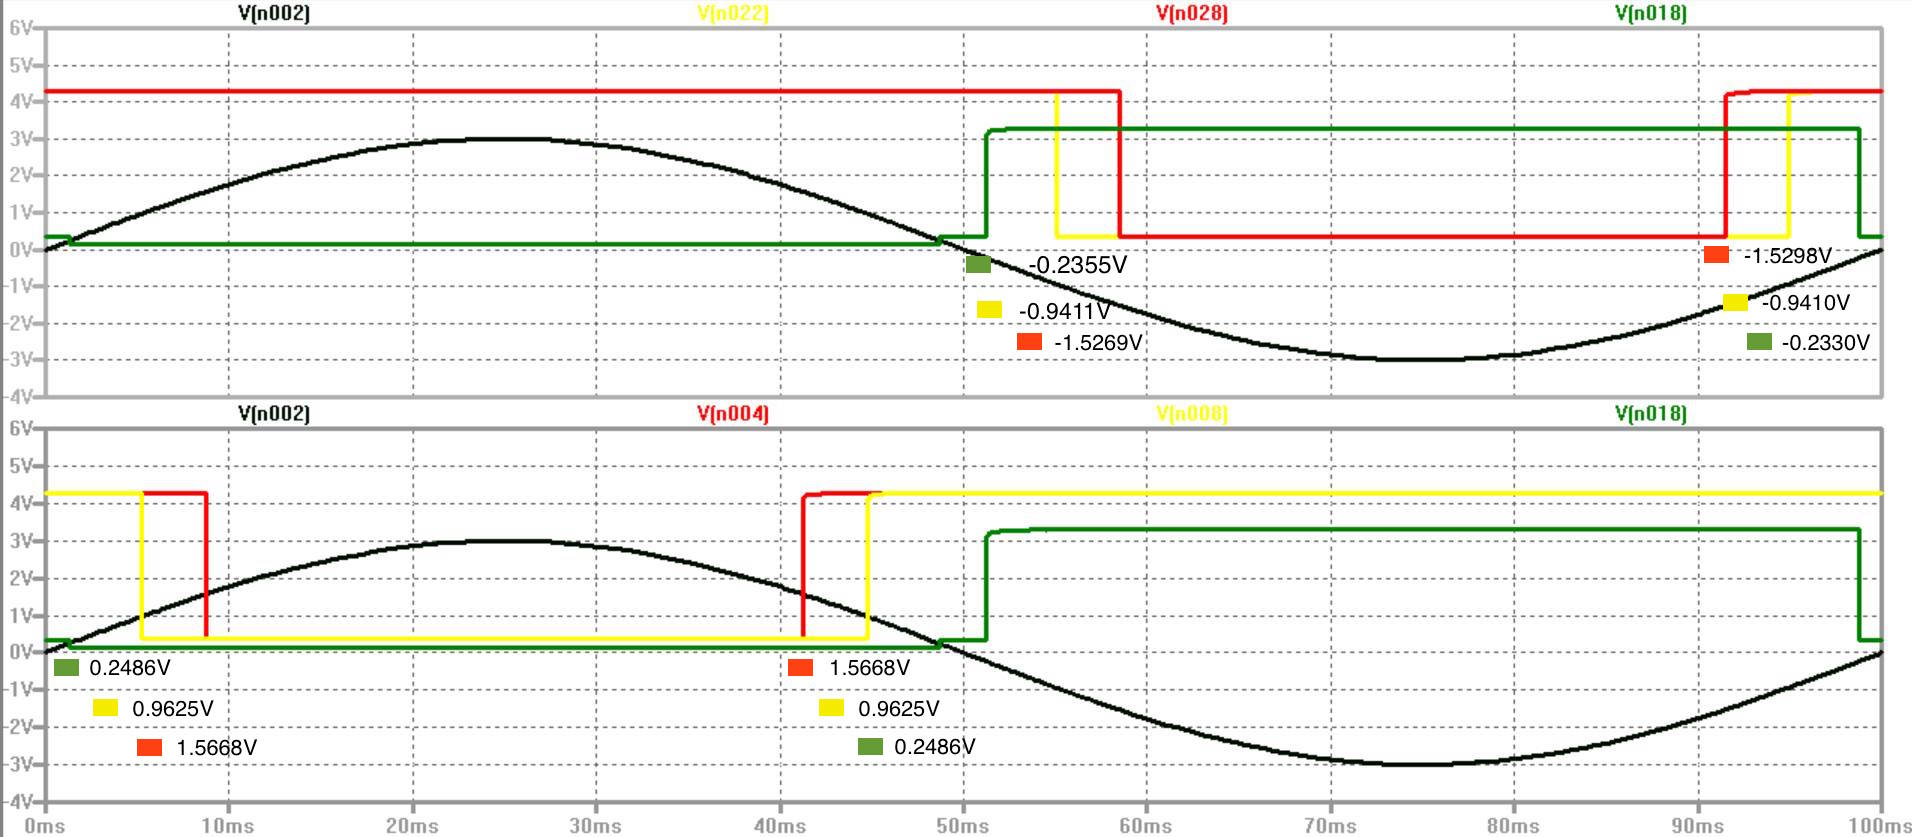
\includegraphics[scale=0.3]{figures/cProblemloesning/komparator_visuel_simulering_samlet1.JPG}
	\caption{På figuren ses simuleringen af den visuelle komparatorkonfiguration. Den sorte kurve er et sinus signal, der illustrerer blokkens inputsignal. De resterende kurver er de enkelte komparatorer, som under tærskelværdien er i negativ mætning. De røde kurver symboliserer den røde diode, de gule kurver de gule dioder og de grønne kurver de grønne dioder. Når inputsignalet når de definerede tærskelværdier, vil kurverne gå i positiv mætning og LED-dioderne vil lyse. Ved vindue-komparatoren er den positive og negative mætning ikke så høj, som ved de normale komparatorer. Dette skyldes, at signalet skal passere yderligere to LED-dioder, hvilket giver et spændingsfald. Kredsløbet er simuleret i LTspice.}
	\label{fig:komparator_visuel_simulering_samlet}
\end{figure}
På figur \figref{fig:komparator_visuel_simulering_samlet} fremgår det, at ved de enkelte tærskelværdier går signalet i positiv mætning, hvilket får LED-dioderne til at lyse. Mætningen er under $5.5$V som er den spænding LED-dioderne maksimalt kan forsynes med  \fxnote{Kontrollere af denne værdi (5.5) er rigtig}, men samtidig nok til at få dioderne til at lyse tydeligt, hvilket krævede mellem $1.7-1.9$V og $0.02$A. 

\begin{table}[H]
	\centering
	\begin{tabular}{|l|l|l|l|l|l|}
		\hline
					& \textit{Tærskelværdier} 	& \textit{Måling til højre} & \textit{Måling til venstre}		&  \textit{\begin{tabular}[c]{@{}l@{}}Afvigelse\\ for højre\end{tabular}}   &  \textit{\begin{tabular}[c]{@{}l@{}}Afvigelse\\ for venstre\end{tabular}}   \\ \hline
\textbf{$2^{\circ}$} 		& $0.2412$V  				&$0.23815127$V 			&$-0.17571651$V		& $1.3\%$  &$??\%$ \\ \hline
 \textbf{$8^{\circ}$} 		&$0.9648$V					&$0.96551609$V			&$0.96777598$V		& $0.07\%$	&$0.3\%$\\ \hline
\textbf{-$8^{\circ}$} 		&-$0.9413$V					&-$0.96784376$V 			&-$0.92251539$V		& $2.8\%$	&$2\%$\\ \hline 		
\textbf{$13^{\circ}$} 		&$1.5679$V 					&$1.5583895$V 		  	&$1.5705552$V		& $0.6\%$	&$0.2\%$\\ \hline
\textbf{-$13^{\circ}$} 		&-$1.5297$VV 				&-$1.5297296$V		   	&-$1.5297259$V		& $0.002\%$	&$0.002\%$ \\ \hline
	\end{tabular}
	\caption{I tabellen ses der, at de anvendte tærskelværdier afviger fra den teoretiske værdi, hvilket er forventet af reelle komponenter. Det er en acceptabel afvigelse, så tærskelværdierne kan derfor anvendes til implementering}
	\label{Tab:Maalingtearskelvaerdier}
\end{table}

Det kan udfra \ref{Tab:Maalingtearskelvaerdier} konkluderes at afvigelsen fra de udregnede tærkselværdier stemmer overens med tolerance for tærkselværdierne jævnfør afsnit \ref{KomparatorAfs}, side \pageref{KomparatorAfs} som var på $\pm1$\%. 

\noindent\textbf{Simulering af somasensorisk komparator kredsløb} \\

\subsubsection{Implementering og test}

%Når referencespændingen er kendt, kan modstandene efter LEDerne bestemmes. Da kredsløbet trækker strøm, har modstandene (R$13$-R$17$) \fxnote{er det de rigtige modstande} til formål at sikre, at spændingsforsyningen ikke drænes. Hvis modstanden er høj, vil strømmen til kredsløbet være lav, og batterierne i spændingsreferencen vil derved holde længere, men hvis modstanden er for høj, kan det have indflydelse på LEDernes lysstyrke. 

Ifølge det valgte design skal der benyttes i alt 21 modstande antal modstande. Ved reelle komponenter vil der være en afvigelse, hvilket fremgår af tabel \ref{Tab:komparator_modstande}. Derudover er det ikke muligt at anvende alle beregnede komponenter, hvorfor der anvendes modstande i serie- og parallelforbindelser. I tabellen vil alle modstandene fremgå, samt den afvigelsen mellem den teoretiske og målte modstand. 
\begin{table}[H]
\centering
\begin{tabular}{|l|l|l|l|}
\hline
\textit{}               & \textit{Teoretisk værdi} & \textit{Målt værdi} & \textit{Afvigelse} \\ \hline
\textit{R1}             & $10$K$\Omega$            & $9.973$K$\Omega$    & $0.27\%$           \\ \hline
\textit{R2}             & $10$K$\Omega$            & $9.992$K$\Omega$    & $0.08\%$           \\ \hline
\textit{R3}             & $10$K$\Omega$            & $9.976$K$\Omega$    & $0.24\%$           \\ \hline
\textit{R4}             & $10$K$\Omega$            & $9.950$K$\Omega$    & $0.50\%$           \\ \hline
\textit{R5}             & $10$K$\Omega$            & $9.985$K$\Omega$    & $0.15\%$           \\ \hline
\textit{R6}             & $10$K$\Omega$            & $9.950$K$\Omega$    & $0.50\%$           \\ \hline
\textit{R7 (Serie)}     & $16.821$K$\Omega$        & $16.758$K$\Omega$   & $0.37\%$           \\ \hline
\textit{R8 (Parallel)}  & $6.285$K$\Omega$         & $6.280$K$\Omega$    & $0.08\%$           \\ \hline
\textit{R9 (Serie)}     & $1068\Omega$             & $1065\Omega$        & $0.28\%$           \\ \hline
\textit{R10 (Serie)}    & $1042\Omega$             & $1036\Omega$        & $0.58\%$           \\ \hline
\textit{R11 (Parallel)} & $6.039$K$\Omega$         & $6.044$K$\Omega$    & $0.08\%$           \\ \hline
\textit{R12 (Parallel)} & $15.765$K$\Omega$        & $15.718$K$\Omega$   & $0.30\%$           \\ \hline
\textit{R13 (Serie)}    & $165\Omega$              & $164.59\Omega$      & $0.25\%$           \\ \hline
\textit{R14 (Serie)}    & $165\Omega$              & $164.54\Omega$      & $0.28\%$           \\ \hline
\textit{R15}            & $100$K$\Omega$           & $99.660$K$\Omega$   & $0.34\%$           \\ \hline
\textit{R16}            & $56\Omega$               & $56.04\Omega$       & $0.07\%$           \\ \hline
\textit{R17 (Serie)}    & $165\Omega$              & $165.07\Omega$      & $0.04\%$           \\ \hline
\textit{R18}            & $100$K$\Omega$           & $99.722$K$\Omega$   & $0.28\%$           \\ \hline
\textit{R19 (Serie)}    & $165\Omega$              & $163.90\Omega$      & $0.67\%$           \\ \hline
\textit{R20}            & $100$K$\Omega$           & $99.628$K$\Omega$   & $0.37\%$           \\ \hline
\textit{R21}            & $100$K$\Omega$           & $99.676$K$\Omega$   & $0.32\%$           \\ \hline
\end{tabular}
\caption{Af tabellen fremgår de teoretiske og reelle værdier for modstandene benyttet i feedbackkonfigurationen for den visuelle del.}
\label{Tab:komparator_modstande}
\end{table}

\noindent Komparatorkonfigurationen testes ved en spændingsforsyning på $5.5$V med et sinussignal som input. Af \ref{Tab: test_reference} fremgår de beregnede og målte tærskelværdier, samt afvigelsen af disse tærskelværdier. 
\begin{table}[H]
	\centering
	\begin{tabular}{|l|l|l|l|} \hline
		& \textit{\begin{tabular}[c]{@{}l@{}}Teoretisk\\ reference\\ input\end{tabular}} & \textit{\begin{tabular}[c]{@{}l@{}}Målte\\ reference\\ input\end{tabular}} & \textit{\% afvigelse} \\ \hline
		\textit{$13^{\circ}$}  & $1.5758$V                                                                      & $1.5748$V                                                                  & $0.06\%$              \\ \hline
		\textit{$8^{\circ}$}   & $0.9697$V                                                                      & $0.9700$V                                                                  & $0.31\%$              \\ \hline
		\textit{$2^{\circ}$}   & $0.2424$V                                                                      & $0.2427$V                                                                  & $0.12\%$              \\ \hline
		\textit{-$2^{\circ}$}  & -$0.2359$V                                                                     & -$0.2373$V                                                                 & $0.59\%$              \\ \hline
		\textit{-$8^{\circ}$}  & -$0.9495$V                                                                     & -$0.9492$V                                                                 & $0.03\%$              \\ \hline
		\textit{-$13^{\circ}$} & -$1.5332$V                                                                     & -$1.5418$V                                                                 & $0.56\%$        \\ \hline     
	\end{tabular}
	\caption{Af tabelle fremgår de teoretiske og målte tærskelværdier ved de enkelte hældningsgrader. Derudover er der beregnet afvigelsen af den teoretiske og målte tærskelværdi.}
	\label{Tab:test_reference}
\end{table}
Jævnfør kravspecifikationerne afsnit \ref{KomparatorAfs} på side \pageref{KomparatorAfs} overholder de målte tærskelværdier tolerancekravet på $\pm1\%$. For at undersøge, hvornår LEDerne og vibratorerne tænder og slukker måles på input- og outputsignalet vha. et osciolloskop. I \tableref{Tab:test-taendsluk} fremgår de teoretiske og målte tærskelværdier for hvornår LEDen og vibratorerne tænder og slukker, samt afvigelsen mellem disse tærskelværdier. 

\begin{table}[H]
\centering
\begin{tabular}{|l|l|l|l|l|l|l|}
\hline
                    & \textit{Teoretisk Tænd} & \textit{Målt Tænd}     & \textit{Afvigelse}      & \textit{Teoretisk sluk}              & \textit{Målt sluk}  & \textit{Afvigelse}      \\ \hline
\textit{$13\circ$}  & $<1.5758$V              & $1.6000$V              & $1.5357\%$               & $>1.5758$                            & $1.6000$V           & $1.5357$                \\ \hline
\textit{$8\circ$}   & $<0.9697$V              & $1.0000$V              & $3.1246\%$               & $>0.9697$V                           & $0.9600$V           & $1.0000\%$               \\ \hline
\textit{$0\circ$}   & -$0.2359 - 0.2424$      & \begin{tabular}[c]{@{}l@{}} -$0.2400$\\ og $0.2800$V\end{tabular} & \begin{tabular}[c]{@{}l@{}}$1.7380\%$\\ og $15.5115\%$\end{tabular} & \begin{tabular}[c]{@{}l@{}}<-$0.2359$\\ og $\textgreater0.2424\%$\end{tabular} & \begin{tabular}[c]{@{}l@{}}-$0.240$\\ og $0.280$\end{tabular} & \begin{tabular}[c]{@{}l@{}}$1.7380\%$\\ og $15.5115\%$\end{tabular} \\ \hline
\textit{-$8\circ$}  & $<$-$0.9495$V           & -$0.9200$V             & $3.1069\%$               & $>$-$0.9495$V                        & -$0.9200$V          & $3.1069\%$               \\ \hline
\textit{-$13\circ$} & $<$-$1.5332$V           & -$1.5300$V             & $0.2087\%$               & $>$-$1.5332$V                        & -$1.5400$V          & $0.4435\%$               \\ \hline
\end{tabular}
\caption{Af tabellen fremgår det, hvornår LEDerne teoretisk bør slukke og tænde og hvornår de blev målt til at tænde og slukke.}
\label{Tab:test-taendsluk}
\end{table}

De teoretiske værdier for, hvornår LED bør slukke og tænde afviger fra de målte værdier. Under testen blev der anvendt et osciolloskop til at måle, hvornår der sker et spændingsfald over LEDerne og gruppen observerede, at osciolloskopet havde en dårlig opløsning og derudover afrundede værdierne, så disse ikke blev særlig præcise. Eftersom der ses så stor en afvigelse mellem de teoretiske og målte værdier anvendes en computer til at teste feedbackkonfigurationen.????? 
